\documentclass[rfvlsi_template_jrnl.tex]{subfiles}
\begin{document}

\section{Introduction}
% The very first letter is a 2 line initial drop letter followed
% by the rest of the first word in caps.
% 
% form to use if the first word consists of a single letter:
% \IEEEPARstart{A}{demo} file is ....
% 
% form to use if you need the single drop letter followed by
% normal text (unknown if ever used by IEEE):
% \IEEEPARstart{A}{}demo file is ....
% 
% Some journals put the first two words in caps:
% \IEEEPARstart{T}{his demo} file is ....
% 
% Here we have the typical use of a "T" for an initial drop letter
% and "HIS" in caps to complete the first word.

%Based on the discussions in Section II, we categorize those architectures according to their idealistic design concepts. 

\IEEEPARstart{T}{his} document serves as a starting template for writing IEEE-trans. paper in NCTU, RFVLSI-Lab.

\subsection{First Time Use of Latex}

\begin{enumerate}
  \item Download Miktex, and open package manager. Remember to synchronize package list. 
  \item \textit{Use} \emph{package} \textsc{manager} \uppercase{to} install the following packages: \textbf{(Please note the different fonts in this paragraph on purpose. Please read source files for commands)}
	\begin{itemize}
		\item All IEEE transactions/bibtex packages. (the \textbf{ieeetran}, and \textbf{biblatex-ieee} package)
		\item \textbf{Textcomp}: support some symbols. (the \textbf{was} package)
		\item \textbf{amsmath}: support some maths. 
		\item \textbf{subfiles}: support independent compilable subfiles .tex structure as used in this template. 
		\item \textbf{dblfloatfix}: fixes double column figures ordering problems. (\textbf{dblfloatfix} package.)
	\end{itemize}
\end{enumerate}

\subsection{Useful Commands}

\begin{enumerate}
\item Use: \textbf{\textbackslash textbackslash}: to show \textbackslash
\item Use: \textbf{\textbackslash label\{aaaa\}} inside figure, table, equations, or floats: and use it later with \textbf{\textbackslash ref\{aaaa\}}
\item Use: \textbf{\textbackslash cite\{paperXXX\}} to cite the paper in the *.bib file.  For the item content of *.bib file, please go to IEEEexplore and click download citation with BibTex format.
\end{enumerate}
Please look for useful formats in this document, and read their source files directly.
\begin{figure}[t]
\centering
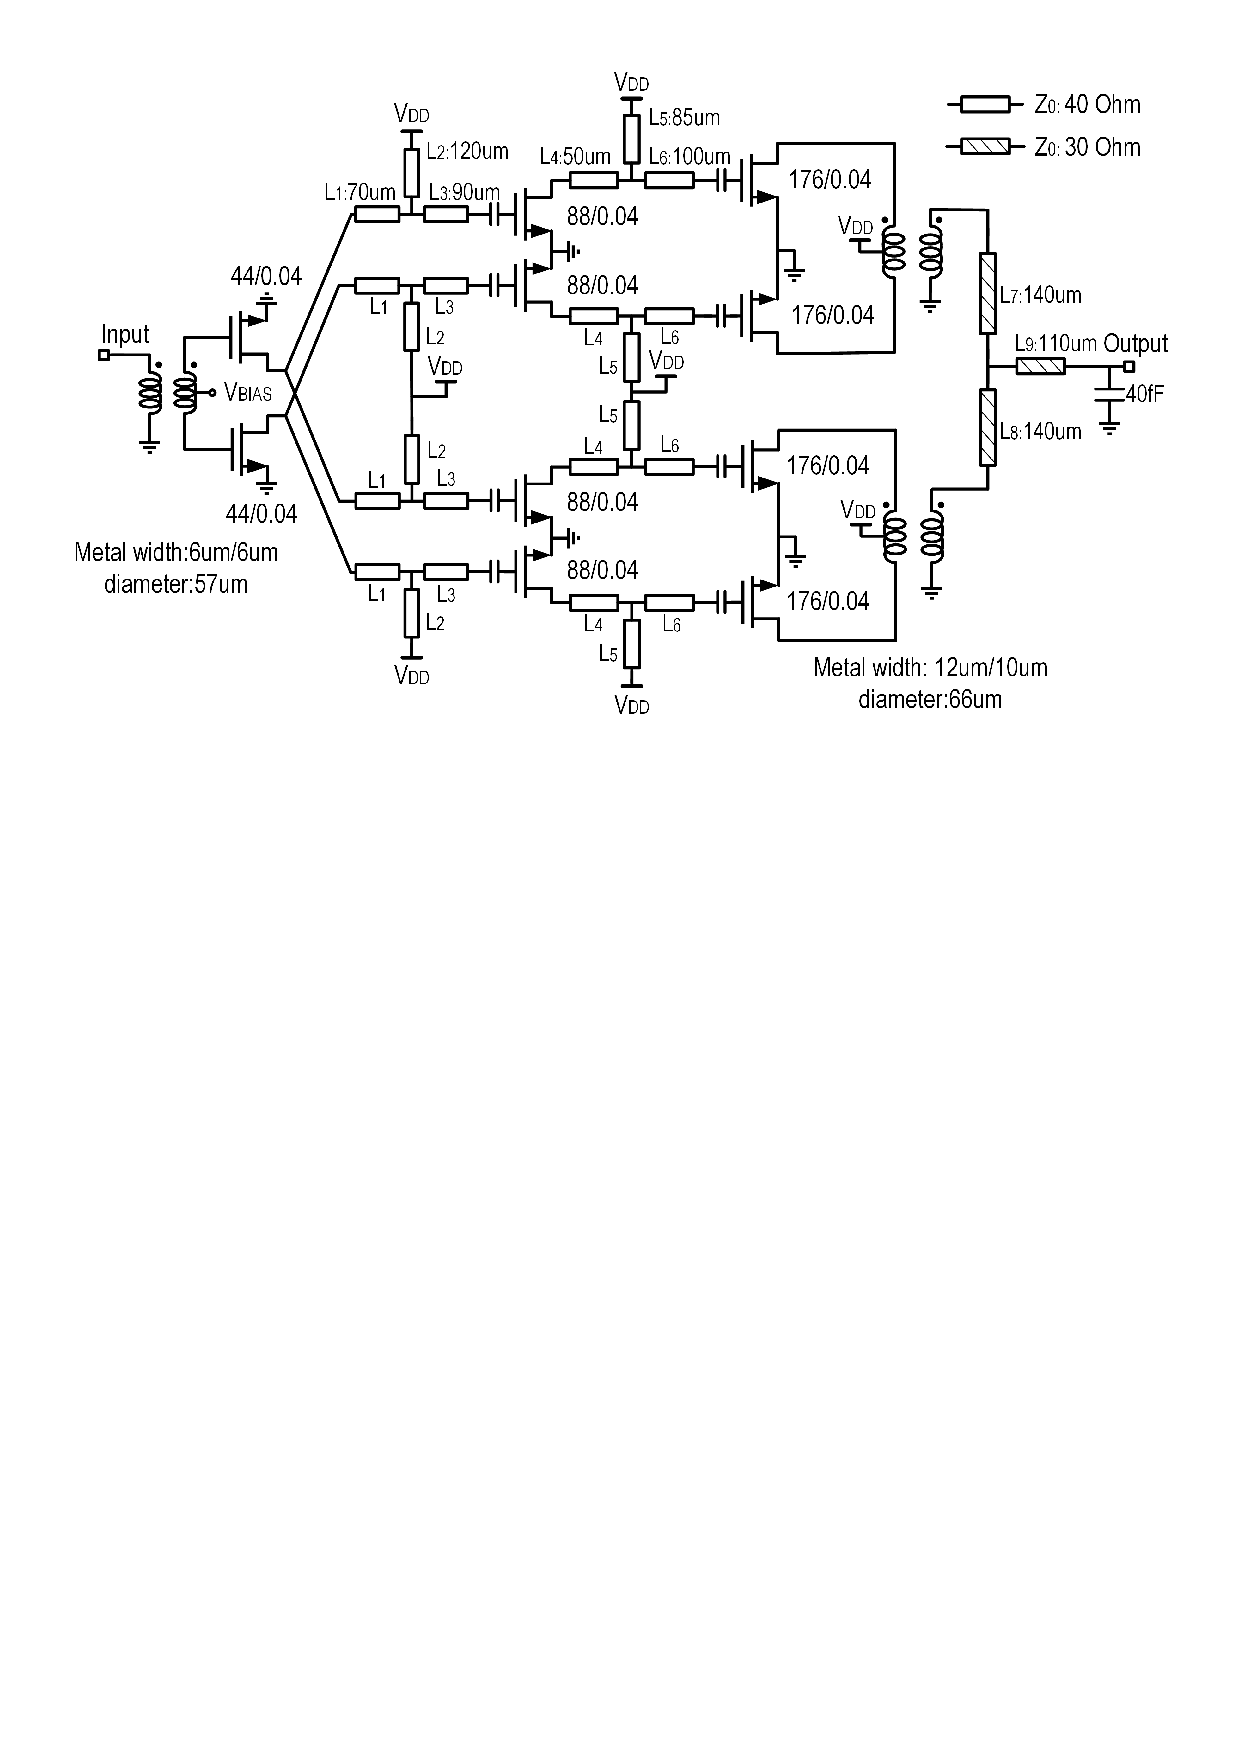
\includegraphics [width=3.6in]{Fig_schematic}
\caption{The simplified schematic of the 60 GHz power amplifier.}
\label{fig:schematic}
\end{figure}

\subsection{Equation Templates }

In all of the following approaches, a gate DC bias $V_{g,bias}$ is introduced as in Eq. XXXX.

\begin{equation}
\label{NStageRectVout}
V_{out}=N⋅(V_{RF,Peak}-V_{th}+V_{gs,bias}).
\end{equation}

Below is a \textbf{IEEEeqnarray} example. Note, it is a 2 by 2 array for alignment.
\begin{IEEEeqnarray}{Rl}
V_G&=A_v\cdot V_{in}-(V_{th}-V_{ITC,bias})\IEEEnonumber\\
&=A_v\cdot \left ( V_{in}- \frac{V_{th}-V_{ITC,bias}}{A_v}\right).
\label{eqn:IGRVgEquation}
\end{IEEEeqnarray}

\subsection{Table Templates}
\begin{itemize}
	\item use \{v/t/v/t/\} to control columns and column separating rule(line). Note that the separating rule are also treated as a column. 
	\item use \newline  \textbf{ \textbackslash IEEEeqnarrayrulerow, \textbackslash IEEEeqnarrayrulerow[rule\_thickness]}, \textbf{ \textbackslash IEEEeqnarraydblrulerow , \textbackslash IEEEeqnarraydblrulerow[rule\_thickness][spacing]}, \textbf{ \textbackslash IEEEeqnarraydblrulerowcut, \textbackslash IEEEeqnarraydblrulerowcut[rule\_thickness][spacing]} to control horizontal separating rules. Use \textbackslash IEEEeqnarraystrutsizeadd\{4pt\}\{4pt\} in the last hidden column in each row to add spaces above/below each row:  \textbf{\textbackslash IEEEeqnarraystrutsizeadd\{4pt\}\{4pt\}}
	\item Use \textbf{\textbackslash parbox\{18ex\}\{\}\}} to control width.
	\item Use \textbf{\textbackslash raggedright}, \textbf{\textbackslash raggedleft}, and \textbf{\centering} to adjust left/right alignment inside each cell.
\end{itemize}
%%%%%%%%%%%%%%%%%%%%%%%%%%%%%%%%%%%%%%%%%%%%%%%%%%
% Summary table for UHF RF-to-DC rectifiers.
\begin{table}[!t]
\centering
\caption{Definition of Sensitivity and Power Conversion Efficiency.}
\label{table_definition}
\centering
\begin{IEEEeqnarraybox}[\IEEEeqnarraystrutmode\IEEEeqnarraystrutsizeadd{2pt}{0pt}][b]{v/t/v/t/v}
\IEEEeqnarraydblrulerow\\
&\textbf{Terminology}&&\textbf{Definition}&\\
\IEEEeqnarrayrulerow\\
&\textit{Power Sensitivity}&&{\parbox{40ex}{The minimum input power required to achieve a specified DC output current, or voltage, or both.}}& \IEEEeqnarraystrutsizeadd{8pt}{8pt}\\
\IEEEeqnarrayrulerow\\
&\textit{Voltage Sensitivity}&&{\parbox{40ex}{The minimum input voltage required to achieve a specified DC output current, or voltage, or both.}}& \IEEEeqnarraystrutsizeadd{8pt}{8pt}\\
\IEEEeqnarrayrulerow\\
&{\parbox{18ex}{\textit{Power Conversion Efficiency (PCE)}}}&&{$PCE\equiv \frac{\text{Output DC power}}{\text{Input RF power}}$} &\IEEEeqnarraystrutsizeadd{4pt}{4pt}\\
\IEEEeqnarrayrulerow
\end{IEEEeqnarraybox}
\end{table}

%Note:
% \IEEEeqnarrayrulerow, \IEEEeqnarrayrulerow[rule_thickness] 
% \IEEEeqnarraydblrulerow , \IEEEeqnarraydblrulerow[rule_thickness][spacing]
% \IEEEeqnarraydblrulerowcut, \IEEEeqnarraydblrulerowcut[rule_thickness][spacing]
% Adding spaces above/below each row:  \IEEEeqnarraystrutsizeadd{4pt}{4pt}
% Use {\parbox{18ex}{}} to control width.
% \raggedright,\raggedleft
%\IEEEpubidadjcol
%
%%%%%%%%%%%%%%%%%%%%%%%%%%%%%%%%%%%%%%%%%%%%%%%%%%
% Summary table for UHF RF-to-DC rectifiers.
\begin{table*}[!t]
\centering
\caption{Summary of the UHF RF-to-DC rectifier performance.}
\label{table_UHF_performance}
\centering
\begin{IEEEeqnarraybox}[\IEEEeqnarraystrutmode\IEEEeqnarraystrutsizeadd{2pt}{0pt}][b]{v/t/V/t/v/t/v/t/v/t/v}
\IEEEeqnarrayrulerow\\
&\textbf{Specification}&&\textbf{This work}&& \textbf{A}&&\textbf{B}&&\textbf{C}&\\
\IEEEeqnarraydblrulerow\\
&{Frequency(MHz)}&&900&& 950&&915&&915&\\
\IEEEeqnarrayrulerow\\

&{Technology}&&\parbox{20ex}{\raggedright 0.28$\mu$m thick-gate oxide CMOS in 65nm process}&& 0.35$\mu$m&&90nm&&0.2$\mu$m&\IEEEeqnarraystrutsizeadd{8pt}{8pt}\\
\IEEEeqnarrayrulerow\\
&{\parbox{19ex}{PCE@Output power}}&&27.97\%@19.3mW&&15.1\%@0.6$\mu$W&&11\%@13.1$\mu$W&&71.5\%@0.285mW&\IEEEeqnarraystrutsizeadd{4pt}{4pt}\\
\IEEEeqnarrayrulerow\\
&{\parbox{19ex}{Number of stage\\/ type of the rectifier}}&&5/half-wave&&\parbox{15ex}{1 (six stacks)\\/ full-wave}&&17/half-wave&&1/full-wave&\IEEEeqnarraystrutsizeadd{4pt}{4pt}\\
\IEEEeqnarrayrulerow\\
&{Chip area}	&&0.442mm$^2$&&0.104mm$^2$&&0.19mm$^2$&&0.133mm$^2$&\\
\IEEEeqnarrayrulerow%
\end{IEEEeqnarraybox}
\end{table*}

%Note:
% \IEEEeqnarrayrulerow, \IEEEeqnarrayrulerow[rule_thickness] 
% \IEEEeqnarraydblrulerow , \IEEEeqnarraydblrulerow[rule_thickness][spacing]
% \IEEEeqnarraydblrulerowcut, \IEEEeqnarraydblrulerowcut[rule_thickness][spacing]
% Adding spaces above/below each row:  \IEEEeqnarraystrutsizeadd{4pt}{4pt}
% \raggedright,\raggedleft
%\IEEEpubidadjcol

%%%%%%%%%%%%%%%%%%%%%%%%%%%%%%%%%%%%%%%%%%%%%%%%%%%%%%%%%%
%%%%%%%%%%%%%%%%%%%%%%%%%%%%%%%%%%%%%%%%%%%%%%%%%%%%%%%%%%
% Comparison table for mmWave RF-to-DC rectifiers.
\begin{table}[!t]
\centering
\caption{Summary of the mmWave RF-to-DC rectifier performance.}
\centering
\begin{IEEEeqnarraybox}[\IEEEeqnarraystrutmode\IEEEeqnarraystrutsizeadd{2pt}{0pt}][b]{v/t/V/t/v/t/v/t/v}
\IEEEeqnarraydblrulerow\\
&&&\textbf{This Work}&&\cite{60GHz_RFID}&& \cite{Gao71GHz2013}&\\
\IEEEeqnarraydblrulerow\\
&Technology&&65nm&&90nm&& 65nm&\\
\IEEEeqnarrayrulerow\\
&\parbox{17ex}{\centering Number of\\ Stages}&&7&&10&&3&\IEEEeqnarraystrutsizeadd{4pt}{4pt}\\
\IEEEeqnarrayrulerow\\
&\parbox{17ex}{\centering Operating Frequency}&&46-56GHz&&45GHz&& 70-72GHz&\IEEEeqnarraystrutsizeadd{4pt}{4pt}\\
\IEEEeqnarrayrulerow\\
&\parbox{17ex}{Peak Efficiency}&&20.65\%&&0.5\%&& 8\%&\\
\IEEEeqnarrayrulerow\\
&Input Sensitivity&&\parbox{17ex}{\centering -6dBm\\@2$\mu$A, 1.2V}&&2dBm&& 5dBm&\IEEEeqnarraystrutsizeadd{4pt}{4pt}\\
\IEEEeqnarrayrulerow%
\end{IEEEeqnarraybox}
\label{table_mmWave_performance}
\end{table}
%Note:
% \IEEEeqnarrayrulerow, \IEEEeqnarrayrulerow[rule_thickness] 
% \IEEEeqnarraydblrulerow , \IEEEeqnarraydblrulerow[rule_thickness][spacing]
% \IEEEeqnarraydblrulerowcut, \IEEEeqnarraydblrulerowcut[rule_thickness][spacing]
% Adding spaces above/below each row:  \IEEEeqnarraystrutsizeadd{4pt}{4pt}


\subsection{Put your own subsections.}
\subsubsection{Put your own subsubsections1.}
\subsubsection{Put your own subsubsections2.}
% You must have at least 2 lines in the paragraph with the drop letter
% (should never be an issue)

\subsection{Online Resources.}
There are many on-line resources for IEEE journal laTex format.  
Please read: \textbf{"How to Use the IEEEtran LATEX Class"} by Michael Shell.
Please read: \textbf{"How to Use the IEEEtran BibTex"} also by Michael Shell.
Please also look for laTex wikiBook for useful tutorials.
% You must have at least 2 lines in the paragraph with the drop letter
% (should never be an issue)

\end{document}

